\section{Técnicas Utilizadas de Data Augmentation} \label{data_augmentation}

Em muitos projetos de Inteligência Artificial, a qualidade e a quantidade dos dados disponíveis têm um impacto direto no desempenho do sistema. Contudo, nem sempre é viável recolher grandes volumes de dados diversificados. Para contornar essa limitação, é comum recorrer a técnicas de \textit{Data Augmentation} (aumento de dados), que consiste em gerar novas amostras a partir das existentes, através da aplicação de transformações específicas.

Esta abordagem permite enriquecer o conjunto de dados original, aumentando a sua variedade e tornando o modelo mais robusto a variações. Assim, o \textit{data augmentation} contribui para melhorar a capacidade do sistema de reconhecer padrões e lidar com situações diferentes das observadas inicialmente.

Para o projeto desenvolvido foram utilizadas as seguintes abordagens de \textit{Data Augmentation}

\subsection{Inserção de Imagens em Fundos Diferentes}

Depois que se mudou de jogo para o \textit{Pokémon HeartGold}, começaram a surgir alguns problemas, onde o modelo detetava botões em locais onde os mesmos não existiam, nem sequer era percetível a presença de um botão nesse lugar. Um exemplo disso são as bordas escuras à esquerda e à direita do jogo, onde o modelo reconhecia botões de combate, apesar de não haver cor nem texto indicativo da presença de um botão. Para um ser humano, é óbvio que ali não poderia estar um botão de combate, mas o modelo estava a identificar padrões que levavam a essa deteção incorreta.

Após algum falar com o professor da disciplina e várias tentativas, percebeu-se que o modelo não estava a aprender a identificar os botões de combate com base na sua cor ou texto, como era o esperado, mas sim apenas pelo seu formato retangular. Por esse motivo, o modelo detetava falsos positivos em regiões onde observava formas semelhantes, como os fundos escuros das bordas.

Para resolver este problema, decidiu-se recorrer a técnicas de \textit{augmentation}, onde os elementos que se pretendem identificar foram recortados e inseridos em fundos de cores diferentes, com o objetivo de forçar o modelo a aprender que os botões devem ser identificados pela sua cor e características visuais, e não apenas pela forma.

Infelizmente, a plataforma \textit{RoboFlow} não disponibilizava este tipo específico de \textit{Data Augmentation} no momento da realização do projeto, pelo que foi necessário realizar este processo manualmente. Os botões foram recortados com o programa de manipulação de imagens \textit{Gimp} e colados sobre diferentes fundos.


\begin{figure}[h]
    \centering
    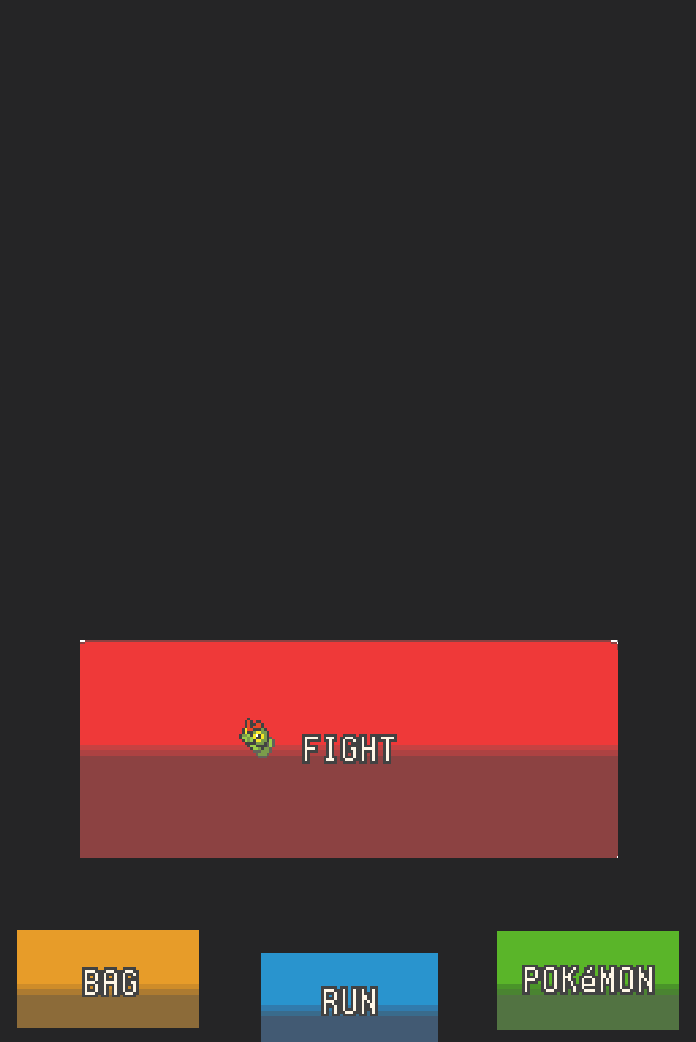
\includegraphics[width=0.5\textwidth]{imagens/augmentation_dark_gray.png}
    \caption{Exemplo de imagem gerada manualmente para \textit{Data Augmentation} no GIMP.}
    \label{fig:data_aug_gimp}
\end{figure}